Las acciones que realiza un vehículo autónomo tienen dos etapas previas bien definidas, la percepción del entorno y el procesamiento de la información adquirida. En este punto se realiza la toma de decisiones, la cual consiste en un conjunto de reglas que imitan el comportamiento del conductor. Su caracterización mediante modelos de toma de decisiones ayuda al desarrollo de algoritmos más naturalistas que impulsen la integración de los vehículos autónomos en el tráfico mixto. 

Los conductores tienen la capacidad de adaptarse a cualquier entorno por muy cambiante que sea, e incluso anticipar ciertas conductas de los vehículos colindantes de manera intuitiva. Por ello, la observación de la estrategia atencional a través del comportamiento de la mirada es capaz de aportar información tanto sobre el estado como de las intenciones del conductor y sus prioridades en la realización de maniobras.

Con objeto de aportar conocimiento sobre esta cuestión, en este capítulo se ha realiza un modelo de conducción determinista focalizado en situaciones potencialmente conflictivas como adelantamientos en vías de alta capacidad. Para ello, se realizan ensayos experimentales en conducción real, emulando diferentes maniobras en función del número de vehículos en el carril izquierdo. Además, se ha adquirido el comportamiento visual a lo largo de los ensayos propuestos, ya que en el \hyperref[ch3]{Capítulo 3} se concluyó que a través de las variables atencionales se pueden determinar patrones o intenciones del conductor en la gestión de la información del entorno.

A continuación, se presenta la estructura del capítulo. En primer lugar, se realiza una encuesta a nivel exploratorio para conocer los aspectos que son considerados más importantes en la toma de decisiones por los conductores. Posteriormente se desarrolla un modelo de conducción clásico de tipo determinista el cual es ajustado y validado con datos de conducción real en una autovía. La obtención de datos del entorno y del conductor ha sido posible gracias a la fusión sensorial presentada en el \hyperref[ch4]{Capítulo 4}.

\section{Encuesta sobre variables en la toma de decisiones}\label{51}
El objetivo de la encuesta es valorar a nivel exploratorio, qué variables consideran más importantes los conductores en la toma de decisiones en conducción. Dichas variables fueron seleccionadas por ser las más comunes en los modelos de conducción, como se observó en el estado del arte del \hyperref[ch2]{Capítulo 2}, siendo evaluadas de manera individual y contraponiéndolas entre sí. 

Las variables analizadas se agrupan en aceleraciones, velocidades, tiempos, otras características y variables abstractas. El vehículo propio se indica con el subíndice 1, el vehículo que le precede con el subíndice 2, y los vehículos adyacentes situados en el carril izquierdo, con los subíndices A, B y C, siendo A el que estaría aproximadamente a la misma altura que el 1, y B y C los que seguirían detrás de A. Las agrupaciones y variables propuestas se detallan en la siguiente tabla \ref{tab:5.1}.

\begin{table}[h]
\centering
\begin{tabular}{rcc}
\textbf{Grupos}                        & \multicolumn{2}{c}{\textbf{Variables}}                                \\ \hline
\multirow{3}{*}{Aceleraciones}         & Aceleración   propia mínima                              & a\textsubscript{1min}    \\ \cline{2-3} 
                                       & Aceleración   propia máxima                              & a\textsubscript{1max}   \\ \cline{2-3} 
                                       & Deceleración   propia máxima                             & dec\textsubscript{1max} 
                                       \\ \hline
\multirow{4}{*}{Velocidades}           & Velocidad   propia                                       & v\textsubscript{1}       \\ \cline{2-3} 
                                       & Velocidad   del vehículo adyacente                       & v\textsubscript{A}       \\ \cline{2-3} 
                                       & Velocidad   media carril izquierdo                       & v\textsubscript{m}       \\ \cline{2-3} 
                                       & Velocidad   máxima de la vía                             & v\textsubscript{max}     \\ \hline
\multirow{3}{*}{Tiempos}               & Tiempo de   seguridad                                    & T          \\ \cline{2-3} 
                                       & Tiempo entre   los vehículos A y B                       & t\textsubscript{AB}      \\ \cline{2-3} 
                                       & Tiempo entre   los vehículos B y C                       & t\textsubscript{BC}      \\ \hline
\multirow{2}{*}{Otras características} & Número de   obstáculos/tráfico                           & n          \\ \cline{2-3} 
                                       & Altura   vehículo delantero                              & h\textsubscript{2}       \\ \hline
Variables abstractas                   & \begin{tabular}[c]{@{}c@{}}Previsión/   Predicción/ Juicios/ \\ Picaresca/ Agresividad\end{tabular} &            \\ \hline
\end{tabular}
\caption{Variables analizadas en la encuesta de toma de decisiones }
\label{tab:5.1}
\end{table}

Los escenarios se resumen en maniobras de seguimiento de vehículo y cambio de carril. La ruta se supone en una vía de alta capacidad, generalmente una autovía o autopista, donde la velocidad máxima son 120 km/h y el trayecto no requiere ningún cambio de ruta. 

La encuesta consiste en un total de 29 preguntas según la escala Likert de 5 opciones y una respuesta abierta, lanzada a través de la plataforma Google Forms. Las preguntas propuestas se encuentran en el \hyperref[AB]{Anexo B: Encuesta sobre variables en la toma de decisiones en la conducción}. Cada cuestión expone una situación de tráfico compleja donde se plantean dos soluciones contrapuestas, cada una priorizando una variable diferente, y donde el conductor debe de determinar el grado de acuerdo con la afirmación. Las preguntas también contemplan una valoración individual de cada variable mediante enunciados en un contexto de tráfico. 

\subsection{Metodología }\label{511}
La muestra se constituye de una total de 120 hombres y 70 mujeres, con edades comprendidas entre 20 y 80 años (\emph{M} = 35.31, \emph{SD} = 12.29). Un 84.21\% de la población manifestó conducir un turismo como vehículo habitual, recorriendo distancias anuales entre 5000 y 10000 km (19.2\%), 10000 y 20000 km (17.54\%) y mayores de 20000 km (63.25\%).

Las puntuaciones obtenidas en la encuesta reflejan la preferencia de los participantes sobre las variables propuestas durante la tarea de conducción. Las variables fueron puntuadas de manera individual y contraponiéndolas entre sí, realizando todas las combinaciones posibles. Las medias de las puntuaciones obtenidas se trasladaron a porcentajes, considerando relevantes los resultados cuya puntuación fuera mayor del 70\%. De igual manera, en los ítems comparativos se consideraron significativas aquellas parejas donde un extremo fuese por lo menos dos tercios mejor valorado que el otro. 

Las preguntas fueron analizadas estadísticamente, atendiendo al tamaño de la muestra y distribución. Dado que en algunos ítems las variables eran valoradas individualmente y en otros se contraponían entre sí, se propuso la evaluación porcentual de las puntuaciones obtenidas, profundizando posteriormente en las más altas. Tras ello, se realizó una matriz de correlación de Pearson con objeto de hallar posibles relaciones entre las variables propuestas. La dinámica de esta prueba se encuentra descrita en el subapartado \hyperref[3111]{3.1.1.1}.

\subsection{Resultados }\label{512}
Las variables mejor valoradas individualmente fueron la aceleración propia mínima (73.68\%) y la velocidad propia (72.52\%), junto a las variables abstractas de predicción (72.95\%) y la previsión (82.11\%). A nivel comparativo se observó que las variables puntuadas más altas frente a otras fueron la velocidad del vehículo adyacente (90.6\%), el tiempo de seguridad (76.21\%) y el tiempo entre los vehículos B y C (73.47\%). Por otro lado, las diferencias significativas halladas en la correlación de Pearson se realizaron en función de los datos demográficos (Tabla \ref{tab:5.2}), obteniendo los siguientes resultados significativos.

\begin{table}[h]
\centering
\begin{tabular}{rcc}
\textbf{Variables}                                                                             & \textbf{\begin{tabular}[c]{@{}c@{}}Coeficiente de correlación\\  Pearson\end{tabular}} & \textbf{Valor \emph{p}} \\ \hline
\textit{Variables individuales}                                                                & \textit{Edad}                               &                  \\ \hline
Aceleración mínima                                                                             & -0.146                                      & 0.045            \\
Aceleración máxima                                                                             & -0,25                                       & \textless{}0.001 \\
Velocidad media carril izquierdo                                                               & -0.266                                      & \textless{}0.001 \\ \hline
\textit{Variables comparativas}                                                                & \textit{Distancia recorrida}                &                  \\ \hline
\begin{tabular}[c]{@{}r@{}}Tiempo de seguridad frente \\ a velocidad propia\end{tabular}       & 0.143                                       & 0.05             \\
\begin{tabular}[c]{@{}r@{}}Velocidad máxima frente \\ altura vehículo delantero\end{tabular} & -0.177                                      & 0.015            \\ \hline
\end{tabular}
\caption{Coeficientes de correlación de Pearson entre variables para toma de decisiones (p\textless{}0.05)}
\label{tab:5.2}
\end{table}

Como se observa en la tabla \ref{tab:5.2}, existe una correlación inversamente proporcional entre la edad y la distancia recorrida con las variables individuales. Dichas variables apuntan a un perfil de conducción más dinámico en los conductores más jóvenes y poco experimentados. En las variables comparativas, los resultados apuntan a que son propensos a sobrepasar la velocidad máxima de la vía con tal de evitar un vehículo de gran altura y que prefieren no modificar su propia velocidad pese a sacrificar el tiempo de seguridad. No se obtuvieron diferencias en relación con los años de experiencia en conducción ni en el tipo de vehículo.

\subsection{Discusión}\label{513}
La toma de decisiones en conducción es un proceso complejo donde intervienen diversas variables, las cuales el conductor analiza y evalúa antes de ejecutar una maniobra. En este apartado se ha propuesto una encuesta para analizar cuáles son las mejor valoradas por los conductores, obteniendo resultados representativos e interesantes.

Comparando las variables entre ellas se obtuvo que la puntuación más alta fue la velocidad del vehículo adyacente, indicando que las acciones de los demás vehículos influyen significativamente sobre las decisiones del conductor. Este hecho está relacionado directamente con la seguridad hacia los demás ya que, si el vehículo circulase completamente solo, primarían más las variables de aceleración propia mínima y velocidad propia, las cuales obtuvieron puntuaciones altas en la evaluación de variables de manera individual. Esta idea se ve reforzada por la alta valoración positiva de las variables abstractas predicción y previsión.

Estadísticamente se encontraron correlaciones entre la edad, distancia anual recorrida y las variables estudiadas. Los conductores más jóvenes valoraron positivamente las variables aceleración propia mínima, máxima y la velocidad media del carril izquierdo, indicando un perfil más enérgico e impaciente. Por otro lado, se encontraron relaciones entre los conductores de largas distancias recorridas y las variables relativas a la seguridad.  Esta conclusión define a estos conductores como pacientes y cautelosos, dado que prefieren evitar las maniobras arriesgadas, aun viendo velocidad menguada, y son conscientes de las capacidades y la dinámica de los vehículos de mayor altura, como pueden ser camiones o autobuses. 

Los resultados obtenidos son interesantes en el desarrollo del modelo de toma de decisiones presentado en el siguiente apartado. Las variables tiempo de seguridad, velocidad propia y velocidad media del carril izquierdo tomarán especial importancia en las decisiones del algoritmo, al igual que se analizarán en detalle la velocidad del vehículo adyacente y los tiempos entre vehículos en las maniobras realizadas.

\section{Modelo determinista para conducción autónoma }\label{52}
En este apartado se presenta el desarrollo de un modelo determinista para conducción basado en un árbol de decisión, cuyas principales acciones son seguimiento de vehículo y cambio de carril. Dicho modelo posee la misma estructura que el sistema de ayuda a la incorporación desarrollado en el subapartado \ref{313}, basado en la aceptación de huecos para la realización de maniobras seguras. 

Las decisiones determinadas por el modelo son dependientes de las variables velocidad, distancia y tiempo de cada vehículo respecto al vehículo propio o ejecutor, 1, donde \emph{v$_2$}, \emph{t$_2$}, \emph{d$_2$} corresponden al vehículo 2 y \emph{v$_i$}, \emph{t$_i$}, \emph{d$_i$}, al vehículo ubicado en el carril izquierdo. Un ejemplo de la disposición de los vehículos puede observarse en la figura \ref{fig:5.1}, donde el vehículo \emph{v$_i$} correspondería a \emph{v\textsubscript{A}}, \emph{v\textsubscript{i+1}} a \emph{v\textsubscript{B}} y \emph{v\textsubscript{i+2}} a \emph{v\textsubscript{C}}.

\begin{figure}[h]
    \centering
    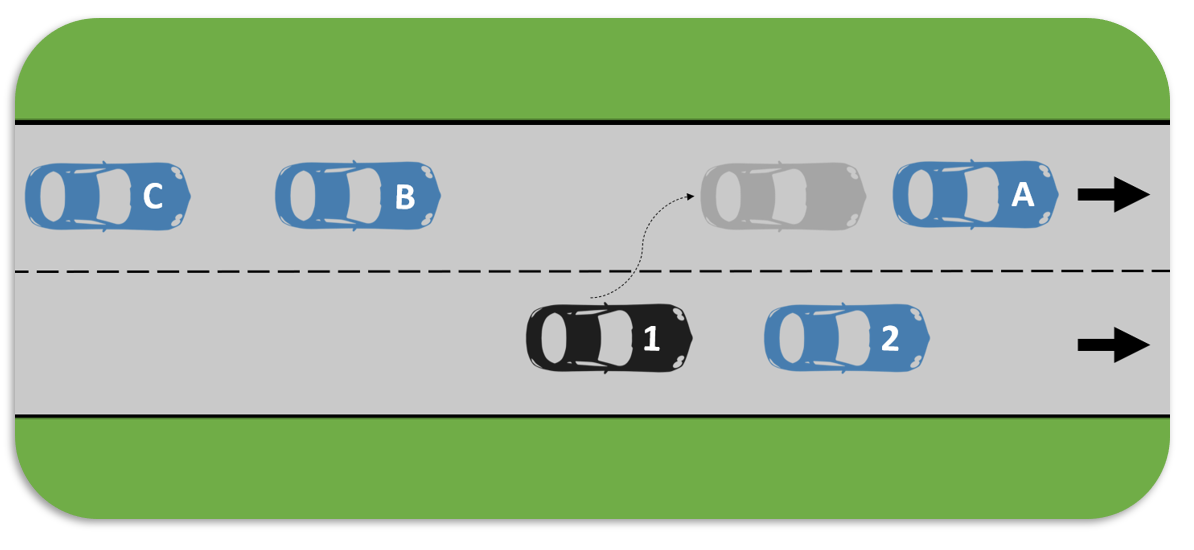
\includegraphics[width=10.5cm]
    {figures/5.1.png}
    \caption{ \label{fig:5.1} Definición de la posición de los vehículos}
\end{figure}

El funcionamiento del modelo se sitúa en el primero de los niveles de abstracción de \textcite{michon}, donde el conductor realiza acciones de planificación sin llegar al nivel táctico donde se ejecutan las órdenes, trabajando con el tiempo de reacción del conductor ante un obstáculo. También se enmarca en las categorías de modelos de seguimiento de vehículos propuestas por \textcite{olstam}, donde el vehículo seguidor mantiene una distancia de seguridad con el vehículo que le precede, reforzando la variable de tiempo de seguridad evaluada en la encuesta de toma de decisiones.

\subsection{Parámetros del modelo}\label{521}
En el modelo de conducción se definen algunos parámetros ajustables, derivados de variables de tiempo y relaciones de velocidades, debido a que en los resultados obtenidos en la encuesta del apartado anterior \ref{51}, los conductores señalaron que las variables más importantes durante la conducción fueron el tiempo de seguridad, la velocidad propia y la velocidad media del carril izquierdo.  

Para el cálculo de los parámetros de tiempo se utilizó la métrica de seguridad tiempo hasta colisión (\gls{ttc}) introducida por \textcite{hayward}, la cual se define como el tiempo necesario para que dos vehículos colisionen manteniendo la misma trayectoria y velocidad. Esta métrica es la relación entre la distancia de seguridad y la diferencia de velocidades de los vehículos y se encuentra relaciona con la fase de predicción en conducción naturalista como se observa en diversos estudios (\cite{li16}; \cite{kilicarslan}; \cite{li22b}). El valor de \gls{ttc} más extendido por la comunidad científica es de 1.5 segundos (\cite{gallelli}, \cite{xu}, \cite{papadoulis}), partiendo de la publicación de \textcite{sayed}, el cual analizó varios valores en función del riesgo, siendo un valor de 1.0 segundos un riesgo alto, 1.5 segundos un riesgo medio y 2.0 segundos un riesgo bajo. Sin embargo, autores más recientes como \textcite{yang20} también contemplaron esta metodología según las características de la vía y la demanda de tráfico, dividiendo de igual manera el riesgo en alto (\gls{ttc} = 1.5 s), medio (\gls{ttc} = 3.5 s), y bajo (\gls{ttc} = 9 s).  

El parámetro tiempo hasta colisión con el vehículo delantero (\emph{t\textsubscript{2}}) es una de las principales variables que define la transición entre los regímenes de circulación propuestos, resumidos en aceleración libre, seguimiento de vehículo, cambio de carril y frenada, para un entorno interurbano (\cite{sharma17}), por lo que en este estudio se utilizará la misma metodología de diferenciación de tiempos en función del riesgo. En los primeros regímenes del algoritmo se distinguen principalmente tres instantes temporales en la variable \emph{t\textsubscript{2}}, los cuales están referenciados al final de la maniobra (Figura \ref{fig:5.2}): 

\begin{itemize}
    \item Tiempo máximo, \emph{t\textsubscript{max}}, que señala el cambio entre aceleración libre y seguimiento de vehículo. 
    \item Tiempo mínimo, \emph{t\textsubscript{min}}, definido por el comienzo de la intención para realizar un cambio de carril. 
    \item Tiempo de seguridad, \emph{T}, el instante en que termina la evaluación del entorno y comienza la ejecución de la maniobra, siendo este tiempo el de seguridad con el vehículo delantero.
\end{itemize}

\begin{figure}[h]
    \centering
    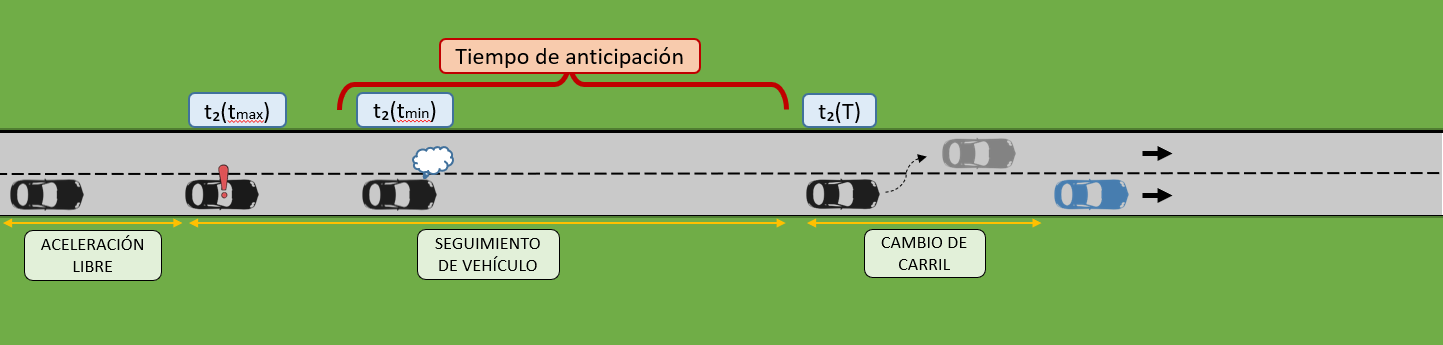
\includegraphics[width=15cm]
    {figures/5.2.png}
    \caption{ \label{fig:5.2} Definición de tiempos en la maniobra de cambio de carril }
\end{figure}

Por otro lado, la velocidad del vehículo respecto a la de los vehículos adyacentes influye directamente sobre la posibilidad de decisión en un entorno, como es el caso de la velocidad media del carril izquierdo, destacada en el apartado anterior. La aparición de la intención de cambio definida en el modelo se encuentra en función de la relación entre alguna de las velocidades propuestas y la velocidad del vehículo propio, siendo estas relaciones la velocidad propia respecto a la máxima de la vía $(v_1/v_{\text{max}})$, la velocidad propia respecto a la velocidad media de los vehículos que circulan por el carril izquierdo $(v_1/v_{\text{m}})$ y la velocidad propia respecto a la del vehículo delantero $(v_1/v_2)$. Una vez generada la intención, el algoritmo daría paso a la valoración del cambio de carril en función de los huecos disponibles. 

Para un correcto funcionamiento del modelo de toma de decisiones, los parámetros mencionados anteriormente serán ajustados con datos recogidos de ensayos experimentales (Tabla \ref{tab:5.3}). Además de los parámetros mencionados, se acotarán otros valores por bibliografía como la velocidad máxima de la vía (\emph{v\textsubscript{max}}), establecida en 120 km/h para turismos que circulan por autovías y autopistas de España, una aceleración máxima posible (\emph{a\textsubscript{max}}) de 1.5 m/s$^2$, con objeto de delimitar el modelo basado en bibliografía conservadora, y una deceleración máxima admisible (\emph{dec\textsubscript{max}}) de 4 m/s$^2$, considerando una frenada cerca de la confortabilidad y sensibilidad alta según algunos autores (\cite{vanarem}; \cite{gartner}; \cite{burgett01}; \cite{naujoks18}).  

\begin{table}[h]
\centering
\begin{tabular}{@{}ccc@{}}
\textbf{Fuentes}              & \multicolumn{2}{c}{\textbf{Parámetros ajustables}}                              \\ \midrule
\multirow{6}{*}{Calculados}   & \textit{T}         & Tiempo de seguridad                               \\ \cmidrule(l){2-3} 
                              & \textit{t\textsubscript{min}}      & Tiempo mínimo                                              \\ \cmidrule(l){2-3} 
                              & \textit{t\textsubscript{max}}      & Tiempo máximo                                              \\ \cmidrule(l){2-3} 
                              & \textit{v$_1$ / v\textsubscript{max}} & \begin{tabular}[c]{@{}c@{}}Relación entre velocidad 1 \\ y la máxima de la vía\end{tabular}           \\ \cmidrule(l){2-3} 
                              & \textit{v$_1$ / v\textsubscript{m}} & \begin{tabular}[c]{@{}c@{}}Relación entre velocidad 1 \\ y la media del carril izquierdo\end{tabular}           \\ \cmidrule(l){2-3} 
                              & \textit{v$_1$ / v\textsubscript{2}} & \begin{tabular}[c]{@{}c@{}}Relación entre velocidad 1 \\ y velocidad de 2\end{tabular}           \\ \cmidrule(l){1-3} 
\multirow{3}{*}{Bibliografía} & \textit{v\textsubscript{max}}      & Velocidad máxima de la vía                                 \\ \cmidrule(l){2-3} 
                              & \textit{a\textsubscript{max}}      & Aceleración máxima del vehículo                            \\ \cmidrule(l){2-3} 
                              & \textit{dec\textsubscript{max}}    & Deceleración máxima del vehículo                           \\ \bottomrule
\end{tabular}
\caption{Parámetros ajustables utilizados en el modelo de toma de decisiones }
\label{tab:5.3}
\end{table}

\subsection{Definición del algoritmo}\label{522}
El algoritmo que compone el modelo de toma de decisiones se basa en una estructura condicional múltiple dentro de una estructura de repetición, contemplando un total de 10 respuestas diferentes, cuyas principales acciones son seguimiento de vehículo y cambio de carril. En función de los huecos disponibles para realizar una maniobra, calculados en base a la información obtenida de los sensores embarcados, el modelo sugerirá la acción más adecuada. Una ventaja que posee este modelo es que su funcionamiento es independiente del número de vehículos participantes, \emph{n}, pudiendo realizar \emph{i}, iteraciones, hasta encontrar un hueco idóneo para realizar la maniobra con seguridad.  

A continuación, se definen los pasos que sigue el algoritmo en la figura \ref{fig:5.3}. El bucle se inicia suponiendo la presencia de un vehículo precedente (vehículo 2) y cuestionando la distancia a la que está: 
\begin{itemize}
    \item Si no hubiera ningún vehículo, o si la distancia fuera lo suficientemente grande, el algoritmo entraría en el primer régimen de circulación, aceleración libre. 
    \item En caso contrario se evalúa la intención de cambiar de carril, condicionada por la velocidad máxima de la vía, \emph{v\textsubscript{max}}, la velocidad media de los vehículos del carril izquierdo, \emph{v\textsubscript{m}}, la velocidad del vehículo 2, \emph{v\textsubscript{2}}, y el tiempo mínimo de inicio de la intención, \emph{t\textsubscript{min}}. Dichas variables soportan los resultados obtenidos en la encuesta del apartado \ref{51}. Si no se cumpliese ninguna condición, el algoritmo seguiría al vehículo 2 y adaptaría su velocidad. 
    \item En caso de adelantar, procedería a la contabilización del número de vehículos situados en el carril izquierdo, \emph{n}, cuyo valor se actualiza en función del flujo de tráfico. El caso más sencillo sería cuando no hay ningún vehículo en el carril izquierdo, \emph{n} igual 0, donde se produciría un adelantamiento casi instantáneo. 
    \item En caso de haber 1 vehículo, se podría adelantar por delante del vehículo A, por delante acelerando, o por detrás del mismo. En caso de producirse un adelantamiento por delante de manera acelerada, la aceleración necesaria para pasar por delante del vehículo A, \emph{a\textsubscript{1di}}, quedaría acotada por un valor máximo coherente, \emph{a\textsubscript{max}}, y la velocidad con la que llegase delante del vehículo adelantado, \emph{v\textsubscript{fti}}, tampoco debería sobrepasar la máxima de la vía, \emph{v\textsubscript{max}}. Si no se pudiera hacer ninguna maniobra, el bucle finalizaría con la condición de \emph{Seguimiento de vehículo con intención de cambio}, volviendo al inicio hasta que existiera un hueco disponible. 
    \item En caso de haber 2 vehículos o más, se podría pasar por delante del primero, entre el primero y el segundo, o pasar el último de la cola. De la misma manera que anteriormente, en caso de realizar la maniobra acelerando entre el primero y el segundo, se ha de valorar que la aceleración necesaria para pasar por detrás del primero, \emph{a\textsubscript{1ti}}, no sea superior a la aceleración necesaria para pasar por delante del segundo, \emph{a\textsubscript{1d(i+1)}}; que ambas se encuentren dentro de unos límites razonables de aceleración, tanto para la máxima, \emph{a\textsubscript{max}}, como para la mínima, \emph{dec\textsubscript{max}}; y que la velocidad final con la que llegase entre los dos vehículos, \emph{v\textsubscript{ft(i+1)}}, no sea superior a la máxima de la vía. 
    \item Si finalmente no considerase posible realizar la maniobra y hubiese más de 2 vehículos, el modelo volvería al inicio de este último bucle analizando análogamente el hueco disponible entre el segundo y el tercero, el tercero y el cuarto, hasta el máximo de vehículos situados en el carril izquierdo.
    \item En caso de no encontrarlo, volvería al inicio del bucle principal, esperando a que se generase un hueco óptimo al igual que en la condición de \emph{Seguimiento de vehículo con intención de cambio}.  
\end{itemize}


Los datos que alimentan el algoritmo son adquiridos a través de ensayos experimentales, en los que se replicarán las escenas mencionadas anteriormente a través de diferentes maniobras. En los siguientes apartados se detallará el procedimiento de los ensayos y se evaluará el funcionamiento del modelo.

\begin{figure}[htbp]
    \centering
    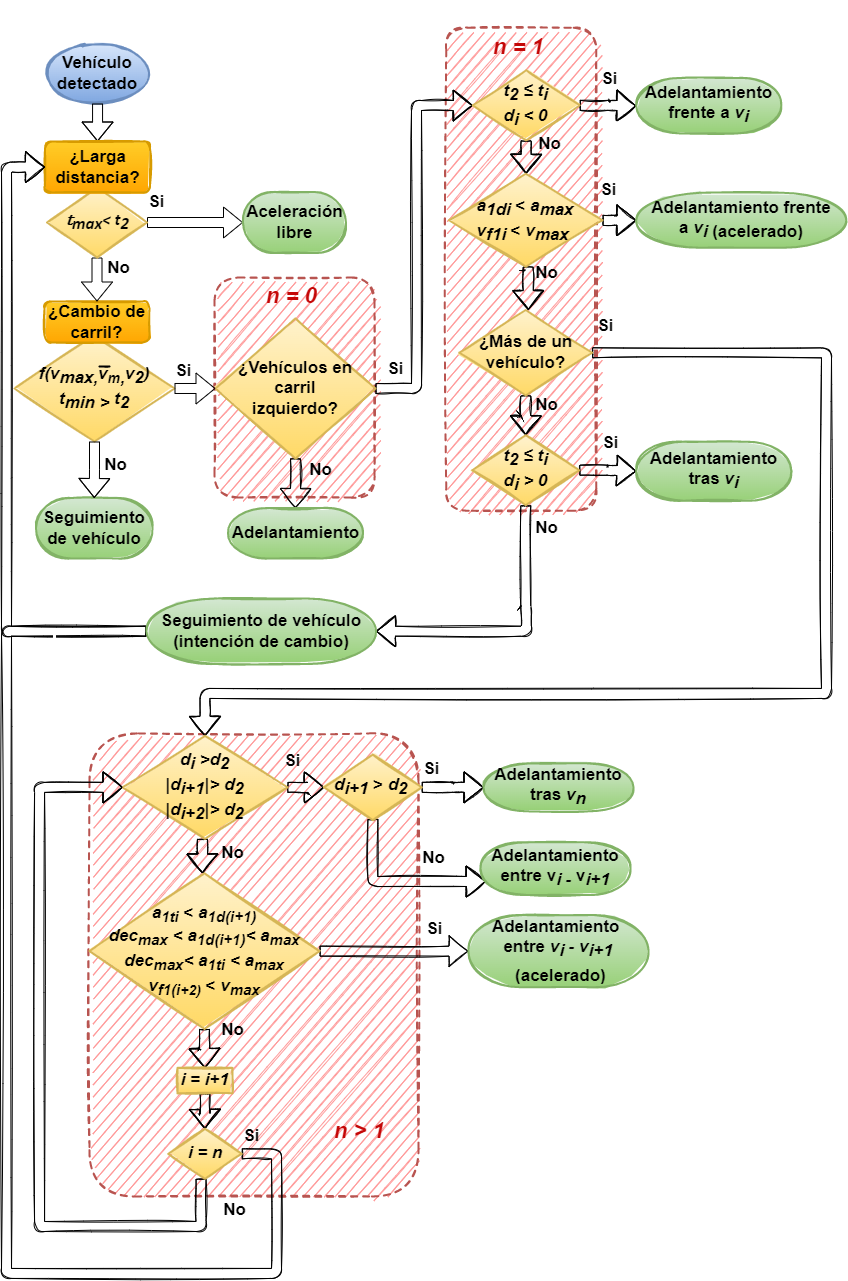
\includegraphics[width=14cm]
    {figures/5.3.png}
    \caption{ \label{fig:5.3} Modelo basado en la aceptación de huecos disponibles}
\end{figure}

\newpage

\section{Ensayos experimentales}\label{53}
Con objeto de validar el funcionamiento del modelo de conducción, se han replicado las maniobras simuladas en tráfico real, alimentando el algoritmo con datos de posición y velocidad de los vehículos participantes, gracias a la instrumentación de un \gls{gps} ubicado en cada vehículo. Los conductores portaron el sistema de seguimiento visual durante las maniobras para el análisis del periodo de anticipación al cambio de carril, con objeto de facilitar la caracterización de esta fase. En el siguiente apartado se muestra la metodología empleada y los resultados concernientes a los ensayos experimentales en diversos ámbitos.

\subsection{Metodología}\label{531}
Un total de 22 ensayos de conducción fueron realizados, correspondientes a 12 hombres y 10 mujeres cuya edad media fue de 33.81 años (\emph{SD} = 6.98). La media de años de experiencia en conducción fue de 14.09 (\emph{SD} = 5.78), siendo el vehículo más utilizado el turismo (68.18\%), seguido de la motocicleta (22.73\%) y los vehículos tipo SUV (9.09\%). La mayoría de los conductores declararon conducir entre 10000 y 20000 kilómetros anuales. Dado que la naturaleza de este estudio está estrechamente ligada a los estilos de conducción, se ha analizado la característica de la impulsividad mediante una encuesta (\cite{perezmoreno}) con la intención de poder abarcar el más amplio espectro de perfiles diferentes y paliando los efectos de la pequeña y homogénea muestra. Esta encuesta se compone de 11 ítems calificando en una escala tipo Likert de 4 opciones. Dicha encuesta también evalúa variables como la agresividad y la impaciencia, sin embargo, para este estudio solo se han analizado las puntuaciones relacionadas con la impulsividad, debido a que este factor se relaciona con la tendencia a realizar maniobras arriesgadas sin considerar las consecuencias a largo plazo, mientras que la agresividad indica expresiones de ira relacionadas con situaciones de tráfico frustrantes, y la impaciencia hace referencia a la falta de tolerancia al tráfico lento.

Los ensayos se realizaron a lo largo de un tramo interurbano de 7.5 km perteneciente a la autovía M-45 de Madrid (Figura \ref{fig:5.4}). La duración total osciló entre 35 y 55 minutos dependiendo del tráfico externo y el número de trayectos necesarios para simular cada caso con seguridad.

\begin{figure}[h]
    \centering
    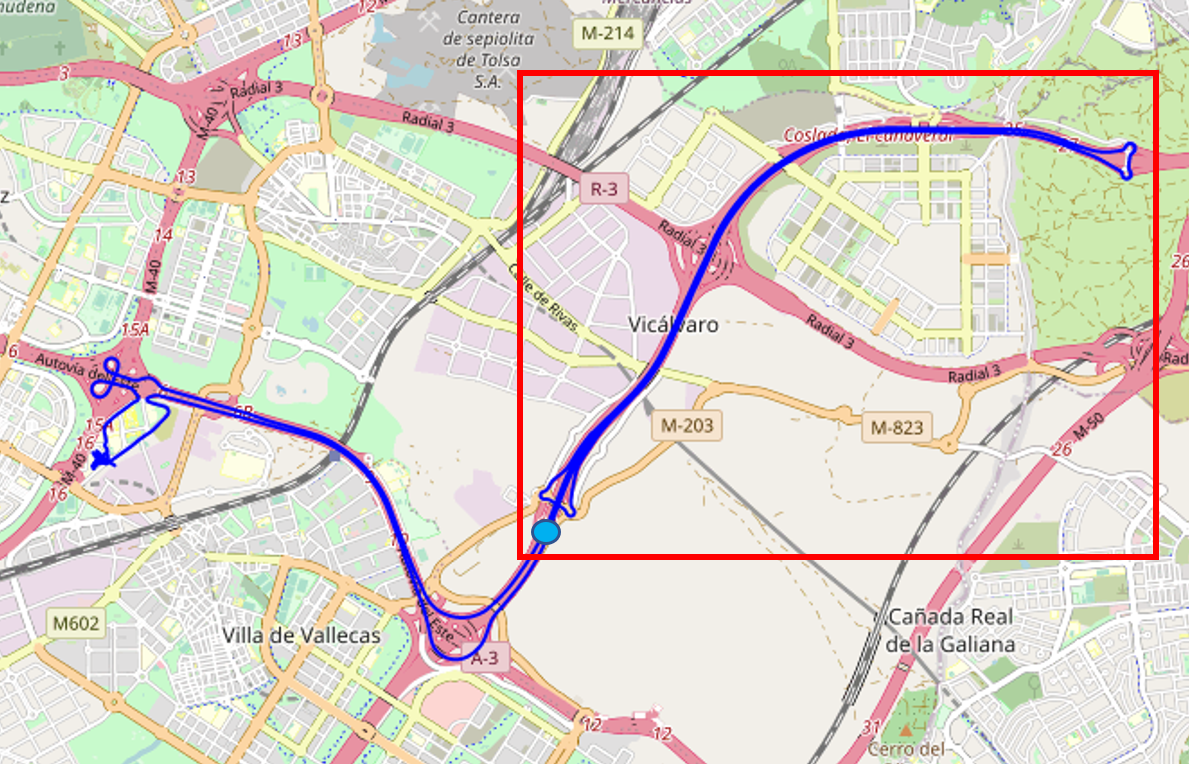
\includegraphics[width=12cm]
    {figures/5.4.png}
    \caption{ \label{fig:5.4} Ruta de conducción en la autovía M-45 (cuadrado rojo) e inicio de la ruta (círculo azul)}
\end{figure}

Cada una de las maniobras planteadas en el algoritmo fueron representadas por el vehículo del participante (vehículo 1), el vehículo precedente (vehículo 2) y tres vehículos ubicados en el carril izquierdo de la vía (vehículos A, B y C), los cuales ajustaban sus velocidades y distancias con objeto de provocar las diferentes situaciones de respuesta del algoritmo (Figura \ref{fig:5.3}). A pesar de que el modelo contempla situaciones donde se requiere una aceleración para el cambio de carril, en los ensayos experimentales no se ha buscado la realización de dichas maniobras por seguridad. Las condiciones quedan resumidas a seguimiento de vehículo con y sin intención de cambio, y los adelantamientos, clasificados como: cambio de carril sin vehículos (C1), cambio de carril delante de A (C2), cambio de carril tras A (C3), cambio de carril entre A y B (C4), cambio de carril entre B y C (C5), y cambio de carril tras C (C6), según corresponde en la Figura \ref{fig:5.1}.

Previo al ensayo se indicó a los participantes que realizasen una conducción lo más natural posible, sin más información para evitar la sugestión en la realización de adelantamientos. La ejecución de las maniobras se efectuó de manera aleatoria, adaptando cada una al tráfico disponible. Los conductores reprodujeron dichas maniobras la mayor cantidad de veces permitida por el tráfico, realizando cada una como mínimo una vez. El diseño del ensayo fue intrasujeto, realizando cada participante todos los casos propuestos como mínimo una vez.

El comportamiento visual se analizó mediante el sistema de seguimiento ocular empleado en el subapartado \hyperref[3121]{3.1.2.1.}, complementado por el sistema de seguimiento de la cabeza desarrollado en el \hyperref[ch4]{Capítulo 4} con objeto de mejorar los datos recogidos de las gafas. El vehículo utilizado por los participantes fue un Peugeot 307 con cambio de marchas automático. Los cinco vehículos fueron instrumentados con un \gls{gps} adquiriendo datos en tiempo real a través del dispositivo M5-Stack, el cual se basa en el SoC (System On a Chip) ESP32 (Figura \ref{fig:5.5}).

\begin{figure}[h]
    \centering
    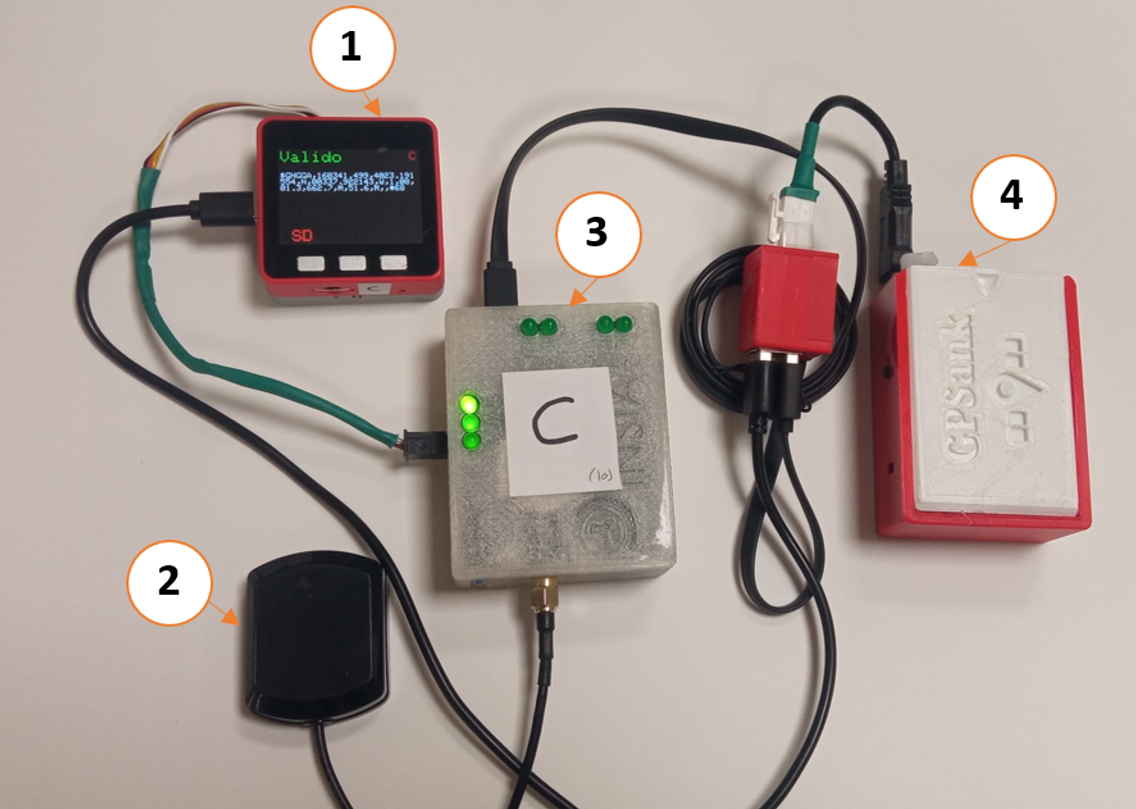
\includegraphics[width=10cm]
    {figures/5.5.png}
    \caption{ \label{fig:5.5} Componentes para la adquisición de datos \gls{gps}. 1. M5-Stack, 2. Antena, 3. \gls{gps}, 4. Sistema de alimentación}
\end{figure}

Los datos sobre la ejecución de las maniobras se muestran de manera descriptiva debido a la diversidad de resultados obtenidos. Además, se buscaron correlaciones entre el diámetro de la pupila y los valores de impulsividad obtenidos de las encuestas sobre perfiles de conducción, a través del coeficiente de Pearson descrito en el subapartado \hyperref[3111]{3.1.1.1.}

\subsection{Resultados} 
El análisis de la encuesta sobre impulsividad durante la conducción se resume en resultados de la figura \ref{fig:5.6}, observando que la muestra es equilibrada, siendo su valor medio 4.78 sobre 10 y su desviación típica 1.43. 

\begin{figure}[h]
    \centering
    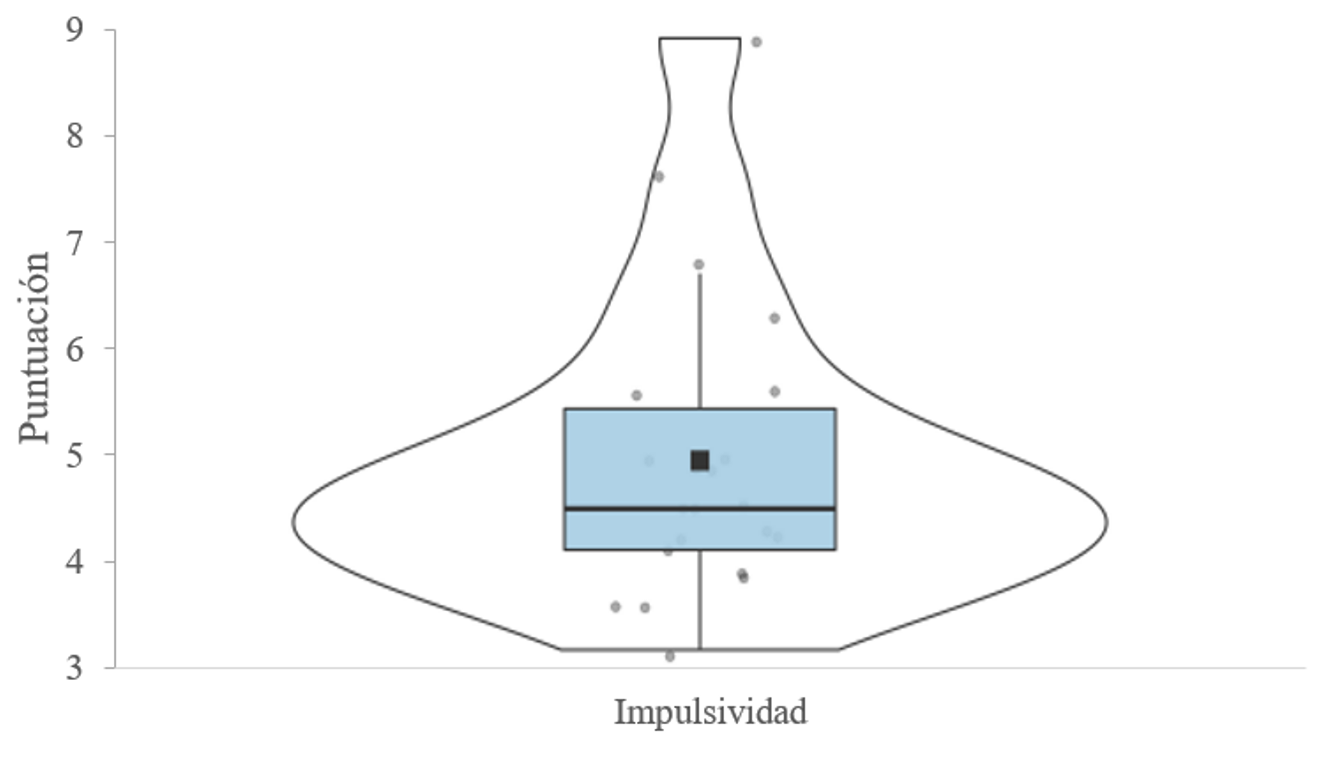
\includegraphics[width=10cm]
    {figures/5.6.png}
    \caption{ \label{fig:5.6} Resultados de impulsividad de la muestra de conductores}
\end{figure}

En la adquisición de datos, un participante no registró datos de \gls{gps} y otros dos tuvieron problemas con el sistema de seguimiento visual, quedando un total de 19 participantes completos. Se plantearon un total de 213 maniobras, repitiendo cada condición una media de 1.87 veces por participante, siendo el caso más repetido C2, pasar por delante de A, y los que menos C5 y C6, pasar entre el penúltimo y el último; y pasar el último de la formación (Figura \ref{fig:5.7}).

\begin{figure}[h]
    \centering
    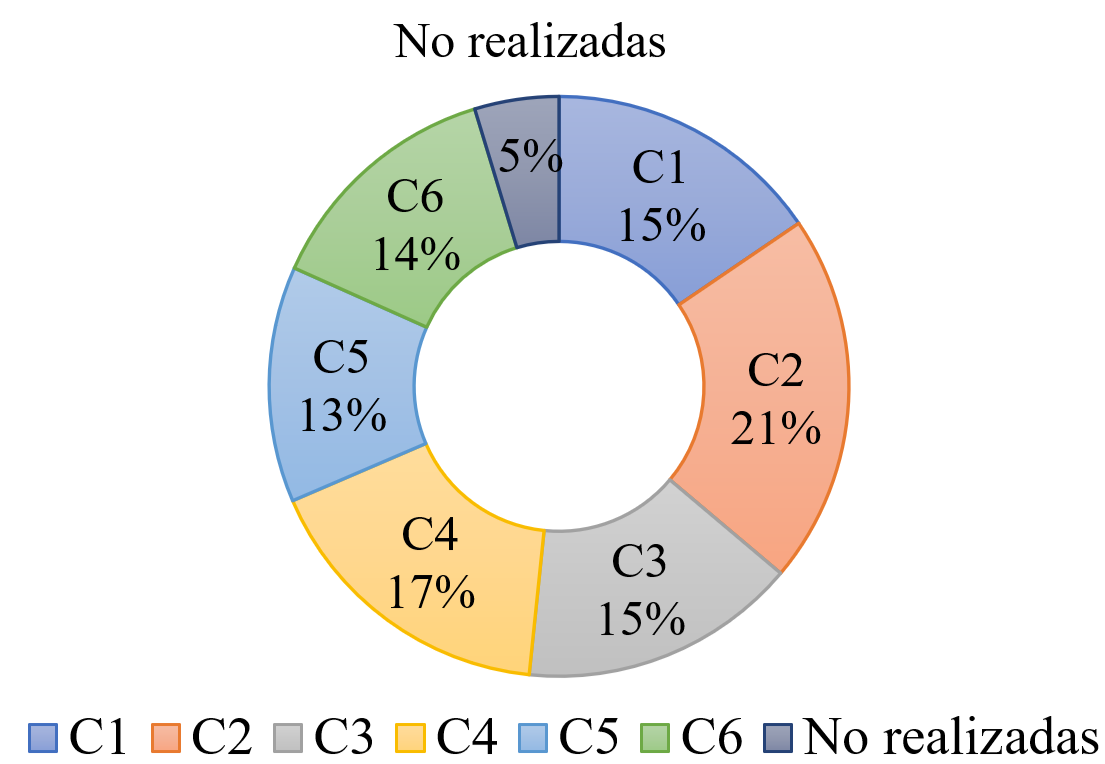
\includegraphics[width=11cm]
    {figures/5.7.png}
    \caption{ \label{fig:5.7} Porcentaje de las condiciones realizadas}
\end{figure}

Del total de las condiciones, hubo un 4.5\% que no se realizaron conforme a la planificación, bien porque el participante decidió no realizar ninguna maniobra, debido en la mayoría de los casos a la intromisión de vehículos externos al convoy del carril izquierdo, o bien porque decidió adelantar antes de que la formación estuviera preparada. 

\textbf{\emph{Hueco disponible en las maniobras}}

La aceptación de hueco en los modelos de conducción es un parámetro determinante en la decisión de maniobras relacionadas con el desplazamiento lateral. Algunos autores diferencian entre hueco hasta el vehículo delantero y hasta el vehículo trasero (\cite{sharma20}; \cite{pakzadnia}), influyendo ambos en la decisión de aceptación o rechazo de la maniobra. Dado que cada maniobra es diferente, se ha estudiado este parámetro en relación con los vehículos adyacentes en el momento de realización del cambio de carril en términos de tiempo. Los resultados obtenidos se muestran en la tabla \ref{tab:5.4}. 

\begin{table}[h]
\centering
\begin{tabular}{@{}cccccccclcclcl@{}}
                                                                           & \multicolumn{2}{c}{\textbf{C2}}               & \multicolumn{2}{c}{\textbf{C3}}               & \multicolumn{2}{c}{\textbf{C4}}               & \multicolumn{3}{c}{\textbf{C5}}                                   & \multicolumn{4}{c}{\textbf{C6}}                                  \\ \cmidrule(l){2-14} 
\multirow{-2}{*}{\textbf{Condiciones}}                                     & \textit{M} & \multicolumn{1}{c|}{\textit{SD}} & \textit{M} & \multicolumn{1}{c|}{\textit{SD}} & \textit{M} & \multicolumn{1}{c|}{\textit{SD}} & \multicolumn{2}{c}{\textit{M}} & \multicolumn{1}{c|}{\textit{SD}} & \multicolumn{2}{c}{\textit{M}} & \multicolumn{2}{c}{\textit{SD}} \\ \midrule
\begin{tabular}[c]{@{}c@{}}Tiempo a vehículo\\  delantero (s)\end{tabular} & \textit{-} & \multicolumn{1}{c|}{-}           & 10.10      & \multicolumn{1}{c|}{5.67}        & 9.91       & \multicolumn{1}{c|}{5.962}       & \multicolumn{2}{c}{9.35}       & \multicolumn{1}{c|}{7.19}        & \multicolumn{2}{c}{21.60}      & \multicolumn{2}{c}{12.74}       \\ \midrule
\begin{tabular}[c]{@{}c@{}}Tiempo a vehículo \\ trasero (s)\end{tabular}   & 40.81      & \multicolumn{1}{c|}{29.87}       & -          & \multicolumn{1}{c|}{-}           & 36.424     & \multicolumn{1}{c|}{24.62}       & \multicolumn{2}{c}{41.38}      & \multicolumn{1}{c|}{37.62}       & \multicolumn{2}{c}{-}          & \multicolumn{2}{c}{-}           \\ \midrule
\begin{tabular}[c]{@{}c@{}}Relación \\ delantero-trasero\end{tabular}      & \multicolumn{2}{c|}{\cellcolor[HTML]{C9C9C9}} & \multicolumn{2}{c|}{\cellcolor[HTML]{C9C9C9}} & \multicolumn{2}{c|}{3.68}                     & \multicolumn{3}{c|}{4.42}                                         & \multicolumn{4}{c}{\cellcolor[HTML]{C9C9C9}}                     \\ \bottomrule
\end{tabular}
\caption{Hueco disponible según condición }
\label{tab:5.4}
\end{table}

En las condiciones C4 y C5, las cuales corresponden al cambio de carril entre dos vehículos, se observó que los conductores dejaron más espacio con el vehículo trasero que con el delantero, 3.7 veces más para la condición C4 y 4.4 veces más para C5. Este hecho se observó también en gran parte de las maniobras realizadas, cumpliéndose en el 89.19\% de las maniobras C4 y en el 90.32\% de las maniobras C5.

\textbf{\emph{Comportamiento visual}}

Al igual que en el subapartado \ref{32} del \hyperref[ch3]{Capítulo 3}, el comportamiento ocular reveló ciertos indicadores de preparación cognitiva en el periodo de anticipación al adelantamiento. Se advirtió que segundos previos a realizar la maniobra las miradas al espejo retrovisor izquierdo aumentaron considerablemente, combinadas ocasionalmente con miradas al espejo retrovisor interior. Este aumento de miradas se observó en la mayoría de los adelantamientos, produciéndose en el intervalo de 10 a 20 segundos antes de cruzar la línea central de la carretera (\emph{M} = 13.2547, \emph{SD} = 5.5826). Dado que el número de miradas osciló en función de la ventana temporal estudiada, se calculó el número de miradas por segundo realizadas en cada cambio de carril, obteniendo un promedio de 0.4358 (\emph{SD} = 0.1599). Multiplicando ambos valores, el intervalo temporal de preparación a la maniobra con el promedio de miradas medio al espejo retrovisor se observa que dicho valor se encuentra por debajo de 6, coincidiendo con la siguiente gráfica de frecuencias (Figura \ref{fig:5.8}) donde se muestra la frecuencia de miradas al espejo retrovisor izquierdo en el periodo de anticipación a la maniobra de cambio de carril. Estos datos apoyan los resultados obtenidos en estudios bibliográficos sobre la modelización del cambio de carril en términos de tiempo (\cite{lee04}; \cite{toledo07}; \cite{xia}) y se asemejan en distribución a los resultados mostrados en la figura \ref{fig:3.16a} del \hyperref[ch3]{Capítulo 3}. 

\newpage
\begin{figure}[h]
    \centering
    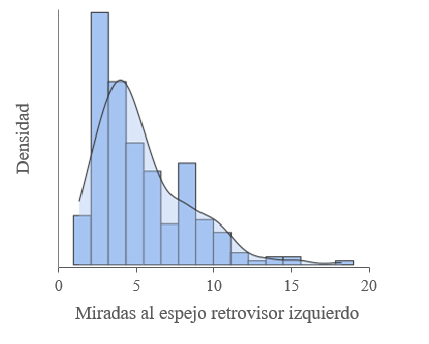
\includegraphics[width=10cm]
    {figures/5.8.png}
    \caption{ \label{fig:5.8} Frecuencia de las miradas al espejo retrovisor izquierdo en la fase de anticipación}
\end{figure}

En relación con el diámetro de la pupila, se ha calculado su valor promedio en función de la maniobra realizada para cada conductor, con objeto de hallar cuales son las condiciones que mayor y menor diámetro de la pupila supusieron para los participantes. Se observa que en el 27.78\% de las condiciones planteadas, el mayor diámetro de la pupila se obtuvo para la condición C1, y en el 38.89\%, el menor diámetro de la pupila se observó en la condición C5. No se obtuvieron correlaciones significativas al analizar la relación entre el valor del diámetro de la pupila por condición y las características obtenidas en la encuesta de perfiles de conducción.

\subsection{Discusión }\label{533}

Los ensayos realizados en tráfico real han sido analizados desde diferentes perspectivas, arrojando resultados interesantes sobre la maniobra de cambio de carril en función de los vehículos situados en el carril izquierdo. Se propusieron un total de seis maniobras, repetidas cada una 1.87 veces en promedio, donde la condición C2, cambio de carril por delante del primer vehículo en el carril izquierdo, fue la más repetida y las condiciones C5 y C6, pasar entre el penúltimo y el último; y pasa el último de la formación, las que menos. Este resultado puede ser debido a la complejidad de estos escenarios, ya que tanto en C5 como en C6 intervinieron todos los vehículos y fueron propensas a que vehículos externos del convoy no sensorizados se intercalasen en la maniobra.  Los resultados en las encuestas de estilos de conducción mostraron que la distribución en las características analizadas es amplia y balanceada, aportando variedad a los resultados.

En relación con el hueco aceptable se observó de manera general que los conductores ajustan su distancia con el vehículo delantero, siendo esta menor que la mantenida con el vehículo trasero y por tanto asimétrica. En las condiciones de cambio de carril entre dos vehículos, C4, entre el primero y el segundo y C5, entre el segundo y el tercero, se obtuvieron resultados interesantes en términos de tiempo hasta colisión con los vehículos adyacentes. Para C4 se calculó que la distancia con el vehículo trasero fue de 3.7 veces mayor que con el delantero, y para C5, 4.4 veces mayor. Estos datos podrían indicar apertura forzada del hueco, consecuente de una desaceleración por parte del vehículo trasero, o un hueco demasiado grande fruto de la posición cooperativa del vehículo trasero, efecto observado en todas las condiciones donde hubo un vehículo detrás en el carril izquierdo.

Respecto al comportamiento visual, se advirtió que un aumento de miradas al espejo retrovisor izquierdo entre los segundos 10 y 20 previos a la realización del adelantamiento es un indicador claro de preparación cognitiva a la maniobra, debido a que esta zona es una de las fuentes principales de información del entorno. Algunos conductores se apoyaron además en el espejo interior, debido a que su apertura permitió un conocimiento global de la escena. Las sucesiones de miradas variaron en función de la complejidad del entorno y el tiempo expuesto, produciéndose una mirada cada dos segundos de manera general. Aunque se obtuvieron situaciones donde el valor mínimo de miradas fue de 1 o 2, se considera que para la predicción de cambio de carril dicho valor debería estar entre 3 y 6, apoyando esta conclusión en el gráfico de frecuencias mostrado en la figura \ref{fig:5.8}.

La maniobra con mayor diámetro de la pupila fue C1, cambio de carril sin vehículos en el carril izquierdo, debido posiblemente a que esta maniobra es la más rápida de todas ya que su entorno es muy sencillo. Por el contrario, la condición C5 fue la que menor diámetro de la pupila supuso para los conductores, cuyo resultado no aporta mucha información a las conclusiones. 

\section{Ajuste de parámetros y validación}\label{54}

El buen funcionamiento del modelo de toma de decisiones planteado se basa en el ajuste de sus parámetros a través de los ensayos experimentales mencionados en el apartado anterior. Para ello, se han calculado dichos parámetros con los datos de conducción de la muestra adquirida y se ha probado su validez comparando las maniobras que tomaría el modelo con las que se realizaron en conducción real bajo las mismas condiciones y en el mismo entorno. Los parámetros a ajustar son instantes de tiempo y relaciones de velocidad.

\subsection{Metodología}\label{541}
Como se mencionaba anteriormente, un total de 22 participantes realizaron ensayos experimentales en conducción real, de los cuales 1 de ellos tuvo problemas en la adquisición de \gls{gps} y 2 en el sistema de seguimiento visual. Para este apartado no se excluyen estos últimos ya que, a pesar de no tener datos del comportamiento visual, sus datos de conducción se consideran válidos para la riqueza de la muestra. Por otro lado, 3 participantes se descartan debido a que globalmente sus valores de impulsividad en conducción muestran valores atípicos, a través del cálculo de la desviación respecto a la media (\emph{D$_i$}). Los participantes descartados mostraron un promedio de las desviaciones respecto a la media superior al 30\%, como se observa en la tabla \ref{tab:5.5}, quedando un total de 18. 

\begin{table}[h]
\renewcommand{\arraystretch}{1.5} % Ajusta el espacio vertical en las celda
\centering
\begin{tabular}{rcccccc}
\multirow{2}{*}{\textbf{Característica}} & \multicolumn{6}{c}{\textbf{Participantes}}  \\ \cline{2-7} 
& \textit{P1}              &  \multicolumn{1}{c|}{\textit{\%D$_{P1}$}} & \textit{P2}              &  \multicolumn{1}{c|}{\textit{\%D$_{P2}$}} & \textit{P3}              &  \textit{\%D$_{P3}$}   \\ \hline
Impulsividad        & 7.5         & \multicolumn{1}{c|}{56.9}           & 8.86        & \multicolumn{1}{c|}{85.4}           & 2.95        & 38.3         \\ \hline
\end{tabular}
\caption{Participantes con valores atípicos de impulsividad en base a la desviación de la media}
\label{tab:5.5}
\end{table}

Debido a que el ajuste de parámetros en el modelo se realiza con valores promedio, se extraen dos participantes de la muestra cuyos valores de impulsividad se encuentren en las zonas más extremas de la muestra, uno con valores bajos y otro con valores altos. La validación de los parámetros ajustables se realizará contra estos dos sujetos, reforzando la validez del modelo independientemente del estilo de conducción por extremo que sea. Para su selección se delimitan las zonas más extremas, eligiendo participantes cuyo promedio de desviación respecto a la media estuviese entre el 15\% y el 30\%, contemplando un total de 5 participantes (Tabla \ref{tab:5.6}).

\newpage
\begin{table}[h]
\renewcommand{\arraystretch}{1.5} % Ajusta el espacio vertical en las celda
\centering
\begin{tabular}{@{}ccccccccccc@{}}
 \multirow{2}{*}{\textbf{Caracteristica}} & \multicolumn{10}{c}{\textbf{Participantes}} \\ \cline{2-11}  & \textit{P4}              & \multicolumn{1}{c|}{\textit{\%D$_{P4}$}} & \textit{P5}              & \multicolumn{1}{c|}{\textit{\%D$_{P5}$}} & \textit{P6}              & \multicolumn{1}{c|}{\textit{\%D$_{P6}$}} & \textit{P7}              & \multicolumn{1}{c|}{\textit{\%D$_{P7}$}} & \textit{P8}              & \textit{\%D$_{P8}$} \\ \midrule
\multicolumn{1}{r}{Impulsividad}            & 3.64                     & \multicolumn{1}{c|}{23.9} & 3.64 & \multicolumn{1}{c|}{23.9} & 3.41 & \multicolumn{1}{c|}{28.7} & 6.14 & \multicolumn{1}{c|}{28.4} & 3.86 & 19.2 \\ \hline
\end{tabular}
\caption{Participantes con valores de impulsividad extremos en base a la desviación de la media}
\label{tab:5.6}
\end{table}

Finalmente, los participantes elegidos para evaluar la bondad del modelo y la idoneidad de los parámetros en las decisiones tomadas para cada maniobra fueron \emph{P6} y \emph{P7}, debido a que en sus porcentajes promedios de desviación respecto a la media se obtuvieron los valores más altos.

Los parámetros estudiados son instantes temporales respecto a la variable \emph{t$_2$} y relaciones de velocidad entre vehículos. Tal y como se mencionó en el subapartado \hyperref[521]{5.2.1. Parámetros del modelo}, el ajuste de tiempos divide en tres parámetros temporales a la variable \emph{t$_2$}, tiempo máximo de aceleración libre, \emph{t\textsubscript{max}}, tiempo mínimo de inicio de la intención de cambio, \emph{t\textsubscript{min}}, y el tiempo de seguridad previo a la ejecución, \emph{T}, referenciados todos al punto final de maniobra.

Para la determinación de cada uno de los instantes temporales, se han observado cambios en las variables obtenidas de los ensayos. El tiempo máximo corresponde al momento en que el vehículo 1 cambia del régimen de aceleración libre a seguimiento de vehículo. Este punto se observa cuando hay un cambio en la velocidad de 1, ya que al ser la velocidad de 2 menor es necesario una reducción para mantener la distancia de seguridad. Cuando el conductor observa un obstáculo en su trayectoria, en este caso el vehículo 2, adopta la actitud de seguimiento de vehículo, situación menos demandante que permite derivar recursos cognitivos a la evaluación del entorno para una toma de decisiones. 

El inicio de esta evaluación puede ser inmediata o no, en función de las necesidades del conductor, y está definida por el tiempo mínimo, que comienza cuando el conductor manifiesta una intención de cambiar de carril. Dicho parámetro se obtiene a través del sistema de seguimiento visual, observando la primera mirada realizada al espejo retrovisor izquierdo para la valoración del entorno. A diferencia de los resultados obtenidos en el apartado anterior \hyperref[53]{5.3 Ensayos experimentales}, \emph{t\textsubscript{min}} es el tiempo hasta colisión con el vehículo 2 (\emph{t$_2$}) en el momento en que comienza la intención de cambio de carril, y el tiempo de anticipación, \emph{t\textsubscript{ant}}, es el intervalo temporal que dedica el conductor a la preparación de la maniobra. 

Por último, el tiempo de seguridad se obtiene observando un aumento de velocidad en el vehículo 1, lo cual indica que se está produciendo un adelantamiento al vehículo delantero. Conjuntamente y tras la definición de los tiempos se calculó la aceleración necesaria del vehículo 1 (\emph{a$_1$}) para la realización del cambio de carril, la cual está acotada entre el tiempo de seguridad, \emph{T}, y el punto final de la maniobra. Este valor ha sido calculado con objeto de respaldar el valor adoptado de bibliografía y aportar conocimiento sobre su variación en cada una de las maniobras propuestas en el cambio de carril.

Las relaciones de velocidad se han calculado en el instante \emph{T}, ya que es en ese punto cuando el conductor comienza a iniciar la maniobra y donde se puede observar como influencia el valor de dichas relaciones, analizando:

\begin{itemize}
    \item La velocidad propia respecto a la máxima de la vía $(v_1/v_{\text{max}})$
    \item La velocidad propia respecto a la media de los vehículos que circulan por el carril izquierdo $(v_1/v_{\text{m}})$
    \item La velocidad propia respecto a la del vehículo delantero $(v_1/v_2)$  
\end{itemize}

La validación se realizará definiendo estos índices en el modelo, que será alimentado con los datos de \gls{gps} de cada uno de los participantes seleccionados y cuyas decisiones en cada maniobra planteada serán comparadas con las que tomaría el modelo en el mismo entorno correspondiendo con el diagrama de la Figura \ref{fig:5.3}. 

Por último, en el modelo se define el número de vehículos situados en el carril izquierdo, \emph{n}, en función de la maniobra simulada, las cuales se introducen en el apartado \ref{531} y se resumen en cambio de carril sin vehículos (C1), cambio de carril delante de A (C2), cambio de carril tras A (C3), cambio de carril entre A y B (C4), cambio de carril entre B y C (C5), y cambio de carril tras C (C6), según corresponde en la Figura \ref{fig:5.1}.

\subsection{Ajuste}\label{542}
Los parámetros a estudiar para su ajuste en el modelo han sido hallados para la muestra de 16 participantes mencionada anteriormente, 18 menos los dos participantes seleccionados para la validación, los cuales son promediados según condición como se muestra en la tabla \ref{tab:5.7}. Adicionalmente se obtuvo el valor de \emph{a$_1$}, el cual se encuentra dentro de los límites de aceleración propuestos en el modelo. 

\begin{table}[h]
\centering
\begin{tabular}{@{}rccccclc@{}}
\multirow{2}{*}{\textbf{Condiciones}} & \multicolumn{2}{c}{\textbf{C1}}          & \multicolumn{2}{c}{\textbf{C2}} & \multicolumn{3}{c}{\textbf{C3}}                  \\ \cmidrule(l){2-8} 
                                      & \textit{M}     & \textit{SD}    & \textit{M}     & \textit{SD}    & \multicolumn{2}{c}{\textit{M}} & \textit{SD}     \\ \midrule
t\textsubscript{max} (s)                              & 46.196         & 31.249         & 38.189         & 21.331         & \multicolumn{2}{c}{63.315}     & 44.050          \\ \midrule
t\textsubscript{min} (s)                              & 36.539         & 20.799         & 31.374         & 18.431         & \multicolumn{2}{c}{51.342}     & 41.241          \\ \midrule
T (s)                                 & 9.454          & 6.022          & 26.531         & 45.723         & \multicolumn{2}{c}{29.700}     & 24.082          \\ \midrule
a\textsubscript{1} (m/s$^2$)                             & 0.286          & 0.141          & 0.295          & 0.131          & \multicolumn{2}{c}{0.444}      & 0.181           \\ \midrule
\multirow{2}{*}{\textbf{Condiciones}} & \multicolumn{2}{c}{\textbf{C4}} & \multicolumn{2}{c}{\textbf{C5}} & \multicolumn{3}{c}{\textbf{C6}}                  \\ \cmidrule(l){2-8} 
                                      & \textit{M}     & \textit{SD}    & \textit{M}     & \textit{SD}    & \multicolumn{2}{c}{\textit{M}} & \textit{SD}     \\ \midrule
t\textsubscript{max} (s)                              & 57.313         & 41.540         & 59.762         & 45.348         & \multicolumn{2}{c}{43.556}     & 27.151          \\ \midrule
t\textsubscript{min} (s)                              & 43.776         & 27.510         & 45.191         & 27.561         & \multicolumn{2}{c}{26.489}     & 11.059          \\ \midrule
T (s)                                 & 25.692         & 18.204         & 36.382         & 24.115         & \multicolumn{2}{c}{18.862}     & 11.561          \\ \midrule
a\textsubscript{1} (m/s$^2$)                             & 0.338          & 0.143          & 0.3811         & 0.153          & \multicolumn{2}{c}{0.4111}     & 0.145           \\ \bottomrule
\end{tabular}
\caption{Parámetros de tiempo y aceleración según condición }
\label{tab:5.7}
\end{table}

En la figura \ref{fig:5.9} se muestra visualmente la proporción que supone cada uno de los tiempos analizados, teniendo en cuenta que se referencian al final de la maniobra siendo este el valor 0.

\begin{figure}[h]
    \centering
    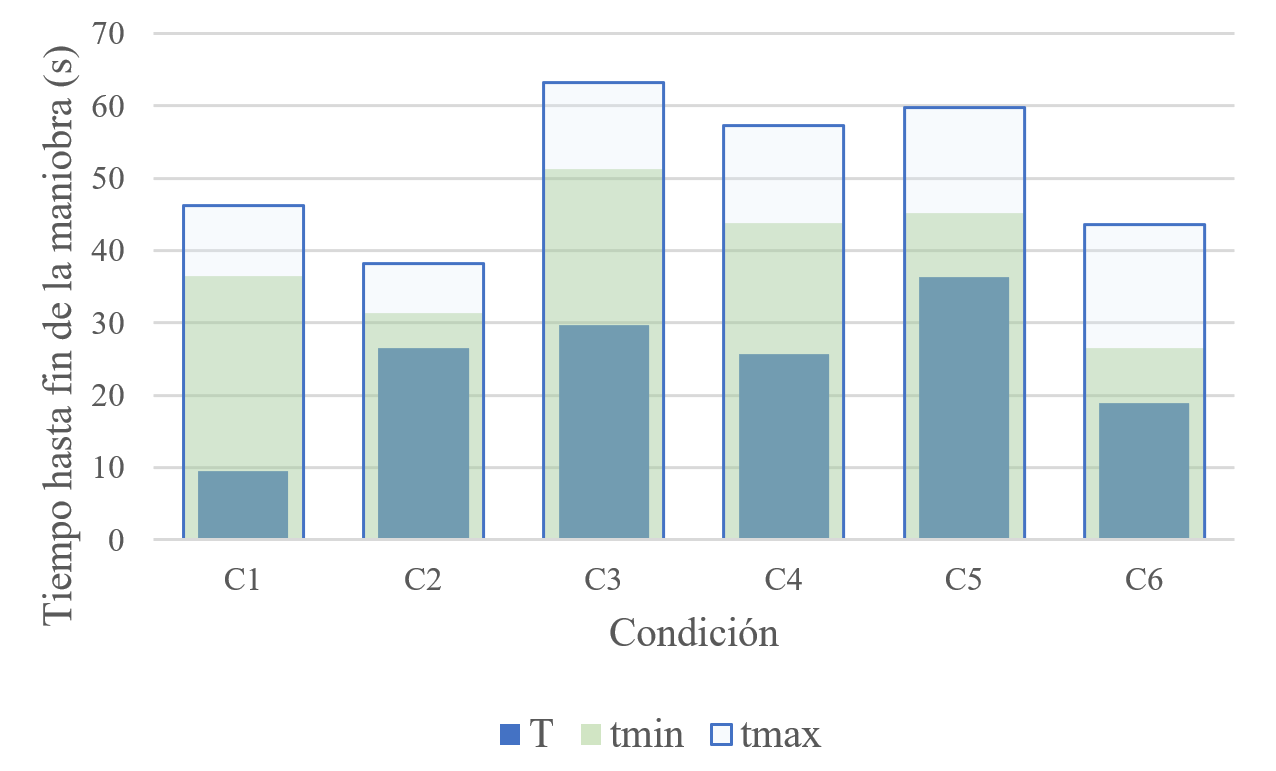
\includegraphics[width=12cm]
    {figures/5.9.png}
    \caption{ \label{fig:5.9} Gráfica de tiempos según condición }
\end{figure}

\newpage
De igual manera, las relaciones de velocidades propuestas para este estudio han sido promediadas y analizadas por condición como se muestra en la tabla \ref{tab:5.8}, mostrándose en valor adimensional. 

\begin{table}[h]
\centering
\begin{tabular}{@{}rccccclc@{}}
\multirow{2}{*}{\textbf{Condiciones}} & \multicolumn{2}{c}{\textbf{C1}} & \multicolumn{2}{c}{\textbf{C2}} & \multicolumn{3}{c}{\textbf{C3}}                  \\ \cmidrule(l){2-8} 
                                      & \textit{M}     & \textit{SD}    & \textit{M}     & \textit{SD}    & \multicolumn{2}{c}{\textit{M}} & \textit{SD}     \\ \midrule
$v_1/v_{\text{max}}$                             & 0.8106         & 0.318          & 0.7659         & 0.308          & \multicolumn{2}{c}{0.7436}     & 0.275           \\ \midrule
$v_1/v_{\text{m}}$                               & 1.0581         & 0.421          & 0.9841         & 0.398          & \multicolumn{2}{c}{0.9386}     & 0.348           \\ \midrule
$v_1/v_2$                               & 1.0968         & 0.428          & 1.0724         & 0.432          & \multicolumn{2}{c}{1.0805}     & 0.399           \\ \midrule
\multirow{2}{*}{\textbf{Condiciones}} & \multicolumn{2}{c}{\textbf{C4}} & \multicolumn{2}{c}{\textbf{C5}} & \multicolumn{3}{c}{\textbf{C6}}                  \\ \cmidrule(l){2-8} 
                                      & \textit{M}     & \textit{SD}    & \textit{M}     & \textit{SD}    & \multicolumn{2}{c}{\textit{M}} & \textit{SD}     \\ \midrule
$v_1/v_{\text{max}}$                              & 0.7058         & 0.271          & 0.6847         & 0.263          & \multicolumn{2}{c}{0.7373}     & 0.246           \\ \midrule
$v_1/v_{\text{m}}$                              & 0.9252         & 0.357          & 0.9277         & 0.360          & \multicolumn{2}{c}{0.9254}     & 0.309           \\ \midrule
$v_1/v_2$                               & 1.0361         & 0.396          & 1.0166         & 0.389          & \multicolumn{2}{c}{1.0766}     & 0.358          \\ \bottomrule
\end{tabular}
\caption{Relaciones de velocidades según condición}
\label{tab:5.8}
\end{table}

El valor promedio de los tiempos y las relaciones de velocidades se implementan en el modelo (Tabla \ref{tab:5.9}), los cuales serán validados por los dos participantes seleccionados a través de sus datos recogidos de \gls{gps}. 

\newpage
\begin{table}[h]
\centering
\begin{tabular}{@{}cclc@{}}
\textbf{}      & \multicolumn{2}{c}{\textit{M}}      & \textit{SD}      \\ \midrule
t\textsubscript{max} (s)       & \multicolumn{2}{c}{51.389} & 10.099           \\
t\textsubscript{min} (s)       & \multicolumn{2}{c}{39.118} & 9.318            \\
T (s)          & \multicolumn{2}{c}{24.439} & 9.294            \\
$v_1/v_{\text{max}}$      & \multicolumn{2}{c}{0.7413} & 0.028            \\
$v_1/v_{\text{m}}$        & \multicolumn{2}{c}{0.9599} & 0.039            \\
$v_1/v_2$        & \multicolumn{2}{c}{1.0632} & 0.027   \\ \bottomrule        
\end{tabular}
\caption{Parámetros de ajuste en el modelo de toma de decisiones}
\label{tab:5.9}
\end{table}

Finalmente se ha estudiando la relación entre los valores de impulsividad obtenidos de la encuesta de perfiles de conducción y los parámetros de ajuste en el modelo, en este caso tiempos. En la figura \ref{fig:5.10} se muestran los valores medios respecto al valor de la impulsividad, obteniendo una regresión de poca calidad debido al limitado tamaño de la muestra de sujetos.

\begin{figure}[h]
    \centering
    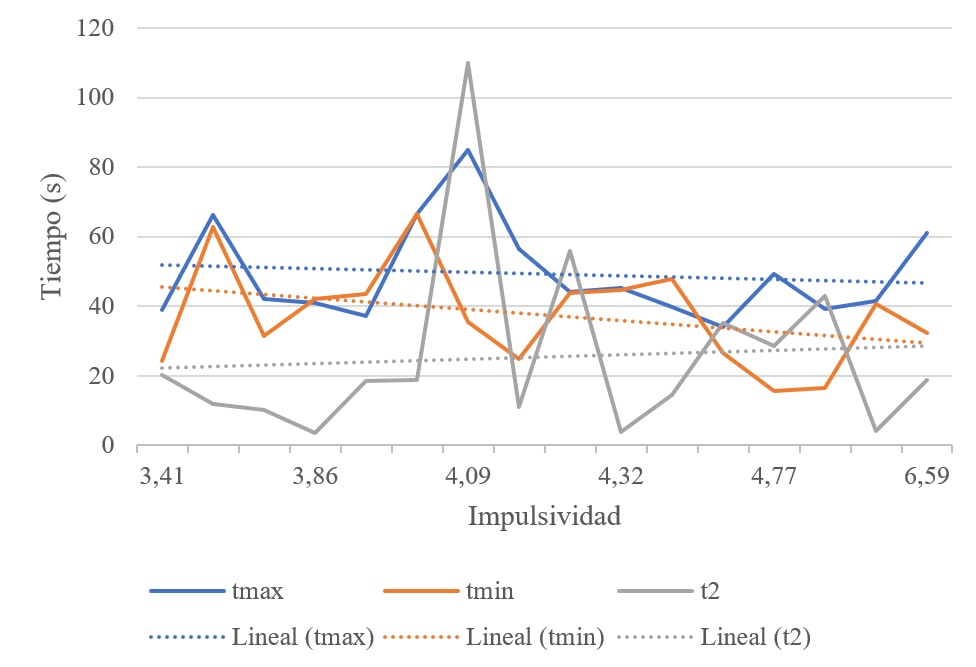
\includegraphics[width=12cm]
    {figures/5.10.png}
    \caption{ \label{fig:5.10} Rectas de regresión de los parámetros de ajuste de tiempo}
\end{figure}

\subsection{Validación} \label{543}
Con el fin de comprobar su validez para todos los casos, se realiza una comparación entre las decisiones de cambio de carril que tomaría el modelo para cada una de las maniobras ensayadas, respecto a las que realizaron los dos participantes analizados, representando cada uno correspondiente un extremo de la muestra total.

Los resultados de coincidencia en función de la maniobra han sido muy satisfactorios como se muestra en la tabla \ref{tab:5.10}. En los casos no coincidentes el modelo sugirió una maniobra cercana a la realizada, posiblemente por la disposición de un hueco previo mejor, realizando la condición C2 en lugar de C3 y C4 en lugar de C5 y C6. En la figura \ref{fig:5.11} se observa la matriz de confusión del total de condiciones con los dos ensayos. 

\begin{table}[h]
\centering
\begin{tabular}{@{}rcccccccc@{}}
\textbf{Condiciones}             & \textbf{Sujetos} & \textbf{C1} & \textbf{C2} & \textbf{C3} & \textbf{C4} & \textbf{C5} & \textbf{C6} & \textbf{TOTAL} \\ \midrule
\multirow{2}{*}{Total}           & \textit{P6}      & 3           & \textit{2}  & 1           & 4           & 1           & 3           & 14             \\ \cmidrule(l){2-9} 
                                 & \textit{P7}      & 2           & 3           & 2           & 3           & 2           & 2           & 14             \\ \midrule
\multirow{2}{*}{No coincidentes} & \textit{P6}      & 0           & 0           & 1           & 0           & 0           & 2           & 3              \\ \cmidrule(l){2-9} 
                                 & \textit{P7}      & 0           & 0           & 0           & 0           & 1           & 0           & 1              \\ \midrule
Tasa de éxito (\%)                        &                  & 100\%       & 100\%       & 66.67\%     & 100\%       & 66.67\%     & 60\%        & 82.22\%        \\ \bottomrule
\end{tabular}
\caption{Resultados de la validación del modelo según condición}
\label{tab:5.10}
\end{table}

\newpage
\begin{figure}[h]
    \centering
    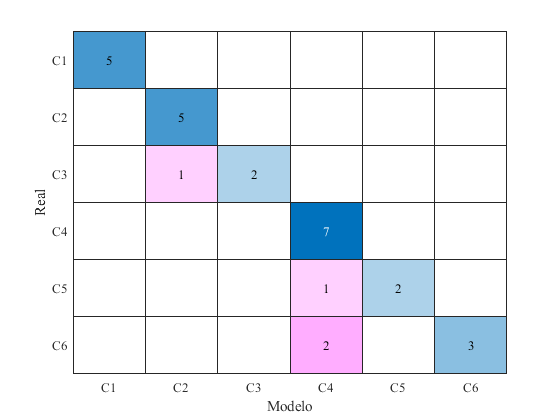
\includegraphics[width=12cm]
    {figures/5.11.png}
    \caption{ \label{fig:5.11} Matriz de confusión de la validación del modelo}
\end{figure}

\subsection{Discusión}
Los parámetros determinantes en la toma de decisiones del modelo de conducción fueron ajustados a través de los datos obtenidos en las maniobras realizadas en tráfico real. Para ello se propusieron tres instantes temporales, los cuales señalaron la detección del vehículo delantero, la evaluación del cambio de carril y la ejecución de la maniobra. En la relación de tiempos por condición, se advierte que en las maniobras C2, C5 y C6, el tiempo de ejecución, correspondiente al segmento entre el margen de seguridad, \emph{T}, y el final de la maniobra, fue mayor en relación al tiempo de anticipación, correspondiente al segmento entre \emph{t\textsubscript{min}} y \emph{T}. Este hecho puede indicar una menor necesidad de análisis del entorno por parte del conductor, bien por impaciencia al cambio de carril, o por facilidad de los vehículos adyacentes a la realización de la maniobra. En la condición C1 el inicio de la ejecución, fue considerablemente menor en proporción al resto de tiempos y a las demás condiciones, siendo este dato muy acertado debido a la simplicidad de este entorno. 

Por otro lado, se observó que, en un gran porcentaje de las relaciones de velocidades propuestas para el inicio de la intención de cambio de carril, la velocidad del vehículo 1 fue menor que la velocidad máxima de la vía y que la velocidad media de los vehículos que circulan por el carril izquierdo, pero mayor que la velocidad del vehículo delantero. Este hecho indica que uno de los principales motivos del cambio es la reducida velocidad del vehículo delantero y la posibilidad de aumentar la propia al igual que los vehículos que circulan por el carril izquierdo.  

Los resultados obtenidos en la comparación de maniobras ejecutadas validaron al modelo con una tasa de éxito del 82.22\% en total. La maniobra menos coincidente fue C6, no por complejidad de la formación como se comentaba en el apartado anterior sino porque el modelo consideró óptimo un hueco más cercano, en este caso la condición C4. Los valores de aceleración necesaria para realizar la maniobra hallados en los ensayos experimentales son acertados en relación a los datos estudiados de fuentes bibliográficas.  

\section{Conclusiones}  

La introducción de la conducción autónoma en el tráfico mixto es un hito social que ayudará a crear un entorno más seguro y fiable para los conductores. Sin embargo, su funcionamiento no solo se basa en una buena percepción, también es necesaria una toma de decisiones realista que contemple el mayor número de reglas posibles y las evalué como lo haría un conductor humano. En este capítulo se han estudiado las variables que más afectan a los conductores durante este proceso y para posteriormente, elaborar un modelo de conducción determinista, basado en la aceptación de huecos del algoritmo del \hyperref[ch3]{Capítulo 3} y enfocado a la toma de decisiones en conducción autónoma. A través de ensayos experimentales se han ajustado y validado dichas variables en el modelo, obteniendo diversos resultados que pueden aportar naturalismo a futuros desarrollos para vehículos autónomos. 

En la encuesta sobre variables significativas en el proceso de decisión, se obtuvieron resultados complementarios a nivel individual y comparativo de las variables propuestas, ya que la prioridad de las mismas depende del número de vehículos ubicados en el carril izquierdo. Individualmente, la aceleración mínima y la velocidad propia fueron las mejor puntuadas, pero comparativamente destacó la velocidad del vehículo que circula por el carril izquierdo por encima de las demás. Este hecho demuestra que los conductores priorizan sus intereses siempre y cuando la velocidad del vehículo adyacente no suponga un riesgo para los mismos, enfatizando en la predicción y la previsión del comportamiento del mismo, variables altamente puntuadas en el grupo de variables abstractas. En base a estos resultados, el modelo de conducción evalúa seis maniobras de cambio de carril con diferentes disposiciones de vehículos en el carril izquierdo.  

Por otro lado, se encontraron diferencias en la determinación de las variables más importantes en función de la edad y la distancia recorrida. A grandes rasgos, los conductores más jóvenes puntúan favorablemente variables que definen una conducción energética e impaciente, como son la aceleración propia, tanto mínima como máxima, y la velocidad media del carril izquierdo. En relación con los conductores de grandes distancias, se observa un comportamiento cauteloso y tranquilo, dado que toleran llevar una velocidad menor a la deseada con tal de no realizar una maniobra precipitada.  

Los resultados obtenidos ayudan a la definición de los parámetros más influyentes en la toma de decisiones en conducción, los cuales se resumen en tiempos de seguridad, en diferentes hitos temporales, y relaciones de velocidades respecto a la velocidad propia. Para ello, se utilizaron datos de ensayos experimentales donde se emularon las seis maniobras propuestas, para posteriormente validar los parámetros calculados con dos participantes seleccionados, cuyos valores de impulsividad se consideran alejados de la media de la muestra. El desarrollo de este apartado permitió realizar varias observaciones sobre las diferencias en la ejecución de las maniobras planteadas.  

Los ensayos experimentales realizados en conducción real aportaron información relevante sobre el comportamiento del conductor en la realización de la maniobra de cambio de carril en diferentes configuraciones de tráfico. En las maniobras de cambio de carril entre dos vehículos se observó que el hueco aceptable no es simétrico entre el vehículo delantero y el trasero, sino que los conductores dejaron más espacio con el vehículo trasero que con el delantero, 3.7 veces más para la condición C4, pasar entre el primero y el segundo, y 4.4 veces para C5, pasar entre el segundo y el tercero. Una posible hipótesis es que la información obtenida a través del espejo retrovisor es indirecta y por tanto los conductores prefieren ajustar su posición respecto al vehículo delantero, en busca de obtener una sensación de mayor control sobre la maniobra. En relación al comportamiento visual, el inicio de la maniobra estuvo marcado por una sucesión de miradas al espejo izquierdo, la cual se produjo entre los segundos 10 y 20 previos al cruce de la línea central de la calzada, y cuyo valor osciló entre 3 y 6 miradas. Los resultados obtenidos permiten caracterizar el inicio de la maniobra de cambio de carril a través del comportamiento visual, siendo esta información relevante en el modelo de toma de decisiones. Los resultados obtenidos sobre el diámetro de la pupila no aportaron información relevante en relación con el estudio realizado.  

En el ajuste de parámetros se observaron diferencias en los parámetros de tiempo en función de la disposición de los vehículos en el tráfico. En las maniobras C2, C5 y C6, el tiempo de anticipación fue comparativamente menor que el tiempo de ejecución, lo cual apuntaba a una evaluación corta del entorno debida a dos posibles hipótesis, una relacionada con el estado del conductor y su necesidad de realizar el cambio de carril cuanto antes, y otra por la posible facilitación de la maniobra por parte del entorno. De igual manera, el tiempo de ejecución en la condición C1 fue más corto en relación al resto, ya que en esta maniobra no había ningún vehículo en el carril izquierdo. En relación a las velocidades, se puede concluir que, en el momento del cambio de carril, el vehículo ejecutor iba más rápido que el vehículo delantero, pero más lento que los vehículos del carril izquierdo y que la velocidad máxima de la vía. 

Finalmente se validaron los parámetros del modelo con los dos participantes propuestos, obteniendo una tasa de éxito del 82.22\% de coincidencia entre las maniobras realizadas por los participantes y las ejecutadas por el modelo. Gracias a la metodología empleada, en este capítulo se han obtenido conclusiones muy coherentes con la realidad, que aportan información interesante sobre cómo afectan diferentes entornos al comportamiento del conductor. Estas contribuciones son respaldadas con resultados empíricos, siendo innovador el análisis del comportamiento visual del conductor aplicado al desarrollo de futuros modelos de conducción naturalistas. 
